\documentclass[]{standalone}
\usepackage{tikz}
\usetikzlibrary{shapes,arrows,calc,positioning}
\usepackage{amsmath} % for dfrac

\tikzset{
    block/.style = {draw, rectangle,
        minimum height=1.2cm,
        minimum width=2cm},
    input/.style = {coordinate,node distance=1cm},
    output/.style = {coordinate,node distance=1cm},
    sum/.style = {draw, circle, node distance=1cm},
}

\tikzset{% from https://tex.stackexchange.com/questions/161075/saturation-block
  saturation block/.style={%
    draw, 
    path picture={
      % Get the width and height of the path picture node
      \pgfpointdiff{\pgfpointanchor{path picture bounding box}{north east}}%
        {\pgfpointanchor{path picture bounding box}{south west}}
      \pgfgetlastxy\x\y
      % Scale the x and y vectors so that the range
      % -1 to 1 is slightly shorter than the size of the node
      \tikzset{x=\x*.4, y=\y*.4}
      %
      % Draw annotation
      \draw (-1,0) -- (1,0) (0,-1) -- (0,1); 
      \draw (-1,-.7) -- (-.7,-.7) -- (.7,.7) -- (1,.7);
    }
  }
}

\begin{document}
        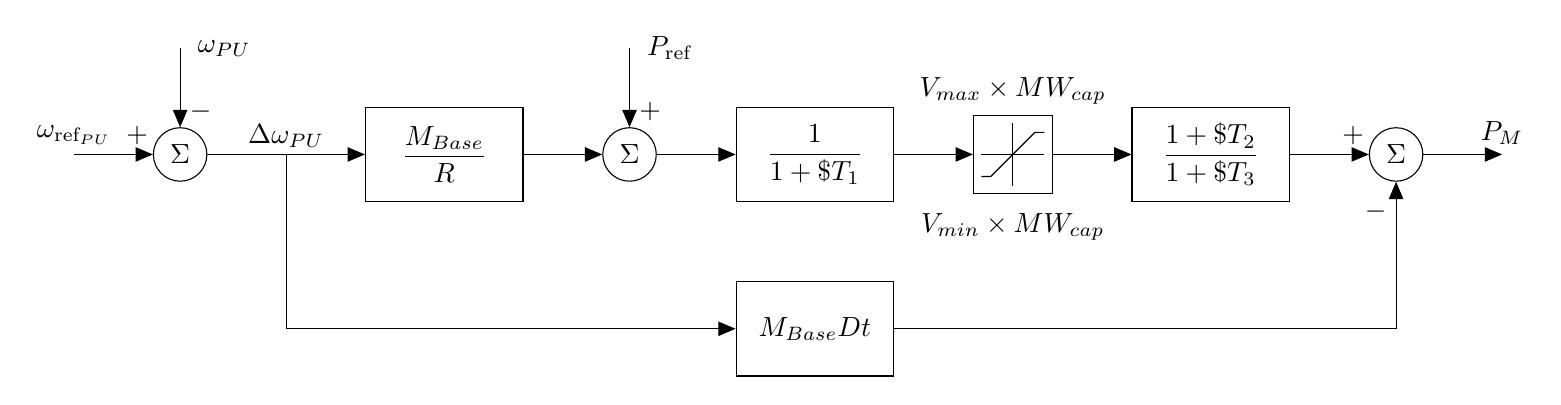
\begin{tikzpicture}[auto, node distance=1cm,>=triangle 45]
        \node [input, name=input, label=$\omega_{\text{ref}_{PU}}$] {};
        \node [sum, right=of input] (sum1) {$\Sigma$};
\coordinate [right=of sum1]  (deltaw) {};
\node [above=-.8em of deltaw,label={$\Delta\omega_{PU}$}]  (deltaWlabel){};
        \node [block, right=of deltaw] (gain) {$\dfrac{M_{Base}}{R}$};
%Add Pref or Pset
\node [sum, right=of gain] (sumP) {$\Sigma$};
        \node [block, right=of sumP] (state1) {$\dfrac{1}{1+\$T_1}$};
\node [block, below=of state1] (Dt) {$M_{Base} Dt$};
%move limiter to here
\node [saturation block, right=of state1 , minimum size=1cm, label=$V_{max} \times MW_{cap}$] (mwcap){};
\node [below=2em of mwcap, label=$V_{min} \times MW_{cap}$](mwcapLOW){};
        \node [block, right=of mwcap] (state2) {$\dfrac{1+\$T_2}{1+\$T_3}$};
        \node [sum, right= of state2] (sum2) {$\Sigma$};

        
        \node [output, right=of sum2, label=$P_M$] (output) {};
        
        \node [input, name=omega, above= of sum1,label={[label distance=.1cm]0:$\omega_{PU}$} ] {};
       	\node [input, name=Pref, above= of sumP,label={[label distance=.1cm]0:$P_{\text{ref}}$} ] {};


        \draw [draw,->] (input) -- node[pos=0.8] {$+$} (sum1);
        \draw [->] (omega) -- node[pos=0.8] {$-$} (sum1);
        \draw [->] (Pref) -- node[pos=0.8] {$+$} (sumP);

        \draw [->] (sum1) -- (gain) ;
        \draw [->] (gain) -- (sumP) ;
		\draw [->] (sumP) -- (state1) ;
        \draw [->] (state1) -- (mwcap) ;
        \draw [->] (mwcap) -- (state2) ;
        \draw [->] (state2) -- node[pos=0.8] {$+$} (sum2);
        \draw [->] (deltaw) |-  (Dt);
\draw [->] (Dt) -|  node[pos=0.9] {$-$} (sum2);
        \draw [->] (sum2) -- (output);
        %\draw [->] (mwcap) -- (output);
        
        \end{tikzpicture} 
\end{document}